\documentclass[10pt,a4paper]{article}
\usepackage[utf8]{inputenc}
\usepackage[spanish]{babel}
\usepackage[margin=1in]{geometry}
\usepackage{amsmath}
\usepackage{amsfonts}
\usepackage{amssymb}
\usepackage{enumitem}
\usepackage{hyperref} 
\usepackage{graphicx}
\usepackage{url}
\usepackage{breakurl}
\hypersetup{pdftex,colorlinks=true,allcolors=black}
\hypersetup{
    pdftitle={},
    pdfauthor={Pablo Riutort Grande},
    pdfsubject={},
    bookmarksnumbered=true,     
    bookmarksopen=true,         
    bookmarksopenlevel=1,       
    colorlinks=true,            
    pdfstartview=Fit,           
    pdfpagemode=UseOutlines,    % this is the option you were lookin for
    pdfpagelayout=TwoPageRight
}
\usepackage{listings}
\usepackage{xcolor}
\usepackage{hypcap}
\definecolor{codegreen}{rgb}{0,0.6,0}
\definecolor{codegray}{rgb}{0.5,0.5,0.5}
\definecolor{codepurple}{rgb}{0.58,0,0.82}
\definecolor{backcolour}{rgb}{0.95,0.95,0.92}
\lstdefinestyle{mystyle}{
    backgroundcolor=\color{backcolour},   
    commentstyle=\color{codegreen},
    keywordstyle=\color{magenta},
    numberstyle=\tiny\color{codegray},
    stringstyle=\color{codepurple},
    basicstyle=\ttfamily\footnotesize,
    breakatwhitespace=false,         
    breaklines=true,                 
    captionpos=b,                    
    keepspaces=true,                 
    numbers=left,                    
    numbersep=5pt,                  
    showspaces=false,                
    showstringspaces=false,
    showtabs=false,                  
    tabsize=2
}
\lstset{style=mystyle}
\usepackage{xparse}
\NewDocumentCommand{\codeword}{v}{%
\texttt{{#1}}
}
\author{Pablo Riutort Grande}
\title{PEC 3\\ \vspace{1cm}\textbf{Reconocimiento de las personas por la imagen de la cara y el iris}}
\begin{document}
\maketitle
\pagebreak
\section{}
Sea \textit{f} el conjunto de matrices formado por (f1,..., f10) y \textit{n} el conjunto de matrices formado por (n1,..., n10)
\begin{enumerate}[label=\textbf{\alph*)}]
\item
\begin{itemize}
\item \textbf{c1}: Los valores de la primera fila son muy similares a los de la matrices f2, f4, f5 y f6. Los valores de la primera columna también tienen muchas similitudes con todas las de las caras excepto con f1. Aunque también existen las mismas similitudes con la matriz n1, dadas las múltiples similitudes con el conjunto \textit{f} y las pocas con el conjunto \textit{n} podría tratarse de una cara.
\item \textbf{c2}: Los valores de esta matriz no son muy similares a ninguna del conjunto \textit{f}, sin embargo, sí que hay muchas similitudes con las del conjunto \textit{n} por lo que podría no tratarse de una cara.
\item \textbf{c3}: Aplicando los mismos criterios de comparación de c1 y dado que estas dos matrices se parecen mucho entre sí, se podría pensar que también se trata de una cara.
\item \textbf{c4}: Esta matriz tiene muy poca similitud con el conjunto \textit{f}, sin embargo, tiene muchas similitudes con las matrices de \textit{n}, en especial con n2, n3, n6, n7 y n10. Por tanto, se puede pensar que no se trata de una cara.
\item \textbf{c5}: Las 3 primeras filas de esta matriz son idénticas a las de la matriz f4, sin embargo las 3 últimas filas son idénticas a las de la matriz n4. ``A ojo'' no es posible deducir si es una cara o no.
\item \textbf{c6}: Las 2 primeras columnas son idénticas a las de la matriz n5 y los demás valors poseen más similitud con el conjunto \textit{n} que con el \textit{f} así que podría ser que no fuera una cara.
\end{itemize}
\item En general, he ido comparando la primera fila y la primera columna de la matriz a clasificar (c) con matrices del conjunto más pequeño (\textit{f}) para encontrar similitudes. He considerado que había suficiente similitud si cada uno de los valores comparados no distaba demasiado de su homólogo en la matriz comparada, es decir, si la diferencia entre ambos valores $c_{ij}$ y $f_{ij}$ era baja.\\
Si no veía mucha similitud entre la matriz c y ninguna del conjunto \textit{f}, entonces, he pasado a buscar similitudes de la misma forma en matrices del conjunto más grande (\textit{n}).
\item Los siguientes valores se han calculado mediante el programa adjunto en el anexo Filtros de Haar[\ref{ann:haar}]
\begin{center}
\begin{tabular}{|c|c|c|c|c|c|c|}
\hline 
 & $C^{1}$ & $C^{2}$ & $C^{3}$ & $C^{4}$ & $C^{5}$ & $C^{6}$ \\ 
\hline 
 $P^{c}_{1}$ & 0.958 & 3.719x10e$^{-12}$ & 0.957 & 2.881x10e$^{-13}$ & 1.759x10$^{-6}$ & 0.916 \\ 
\hline 
$P^{c}_{2}$ & 0.867 & 0.120 & 0.845 & 0.126 & 0.827 & 0.610 \\ 
\hline 
$P^{c}_{3}$ & 0.840 & 0.137 & 0.830 & 0.147 & 0.545 & 0.053 \\ 
\hline 
$P^{c}_{4}$ & 0.958 & 8.266x10e$^{-6}$ & 0.953 & 4.807x10e$^{-5}$ & 0.960 & 0.371 \\ 
\hline 
$\prod\limits_{i=1}^4 P^{c}_{i}$ & 0.669 & 5.076x10e$^{-19}$ & 0.641 & 2.582x10e$^{-19}$ & 7.638x10e$^{-7}$ & 0.011 \\ 
\hline 
$P^{nc}_{1}$ & 0.041 & 0.999 & 0.042 & 0.999 & 0.999 & 0.083 \\ 
\hline 
$P^{nc}_{2}$ & 0.132 & 0.879 & 0.154 & 0.873 & 0.172 & 0.389 \\ 
\hline 
$P^{nc}_{3}$ & 0.159 & 0.862 & 0.169 & 0.852 & 0.454 & 0.946 \\ 
\hline 
$P^{nc}_{4}$ & 0.041 & 0.999 & 0.046 & 0.999 & 0.039 & 0.628 \\ 
\hline 
$\prod\limits_{i=1}^4 P^{nc}_{i}$ & 3.609x10e$^{-5}$ & 0.758 & 5.085x10e$^{-5}$ & 0.744 & 0.003 & 0.019 \\ 
\hline 
Clase & Cara & No cara & Cara & No cara & No cara & No cara\\ 
\hline 
\end{tabular} 
\end{center}
\item Resultados de aplicar únicamente Haar$_{1}$[\ref{ann:haar2}] en el conjunto de imágenes:
\begin{center}
\begin{tabular}{|c|c|c|c|c|c|c|}
\hline 
 & $C^{1}$ & $C^{2}$ & $C^{3}$ & $C^{4}$ & $C^{5}$ & $C^{6}$ \\ 
\hline 
 $P^{c}_{1}$ & 0.958 & 3.719x10e$^{-12}$ & 0.957 & 2.881x10e$^{-13}$ & 1.759x10$^{-6}$ & 0.916 \\ 
\hline 
$\prod\limits_{i=1}^4 P^{c}_{i}$ & 0.958 & 3.719x10e$^{-12}$ & 0.957 & 2.881x10e$^{-13}$ &1.759x10$^{-6}$ & 0.916 \\ 
\hline 
$P^{nc}_{1}$ & 0.041 & 0.999 & 0.042 & 0.999 & 0.999 & 0.083 \\ 
\hline 
$\prod\limits_{i=1}^4 P^{nc}_{i}$ & 0.041 & 0.999 & 0.042 & 0.999 & 0.999 & 0.083 \\ 
\hline 
Clase & Cara & No cara & Cara & No cara & No cara & Cara\\ 
\hline 
\end{tabular}
\end{center}
Al no haber más probabilidades que la correspondiente a Haar$_{1}$ no existe un conjunto de probabilidades que multiplicar y por eso $P^{c}_{1} = \prod\limits_{i=1}^4 P^{c}_{i}$ y $P^{nc}_{1} = \prod\limits_{i=1}^4 P^{nc}_{i}$.\\
Cabe destacar la discrepancia obtenida en la imagen $C^{6}$ donde en el ejercicio anterior fue catalogada como ``No cara'' y esta vez el resultado ha variado a ``Cara'' y, por tanto, no se obtiene la misma clasificación de las seis imágenes.
\end{enumerate}
\section{}

\begin{enumerate}[label=\textbf{\alph*)}]
\item Para este ejercicio se ha utilizado el programa de edición de imágenes Gimp y sus distintas herramientas de selección. Gimp considera el punto origen (0, 0) en el extremo superior izquierdo de la imagen.
\begin{itemize}
\item Estimación del centro pupilar: \textbf{(123, 126)}\\
Para esta estimación se ha creado un cuadrado que contenga a la pupila y se han dibujado sus diagonales. La intersección de estas nos dará el punto que corresponde al centro del cuadrado que coincidirá con el de la pupila.
\begin{figure}[h!]
  \centering
  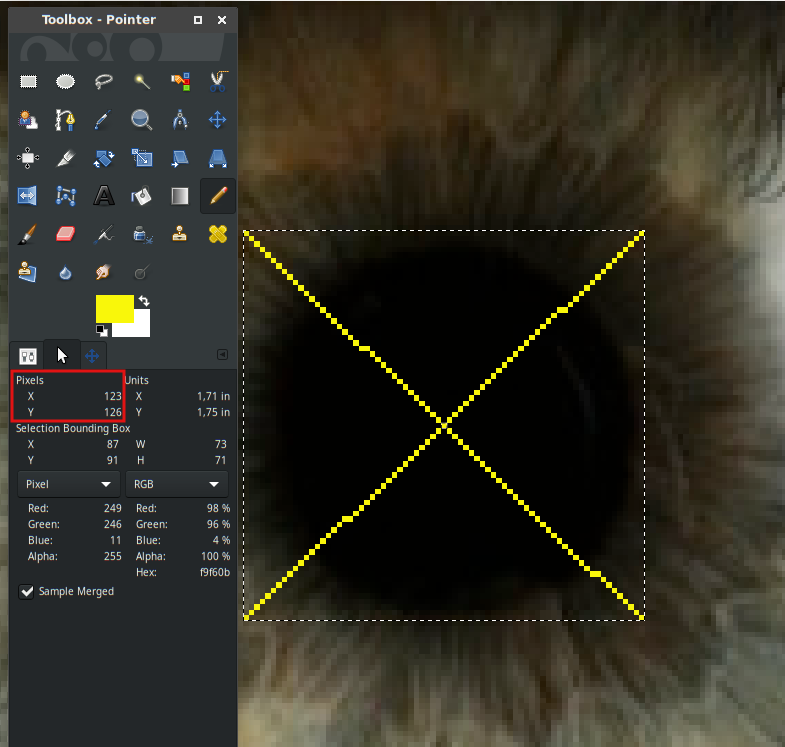
\includegraphics[scale=0.3]{eye1.png}\\
  \caption{Intersección de las diagonales del cuadrado que contiene la pupila nos da el centro pupilar}
  \label{fig:pupil}
\end{figure}
\pagebreak

\item Estimación del radio de la pupila: \textbf{36px}.\\
Esta estimación se ha hecho con la herramienta de Medida de distancias de Gimp y además la coordenada \textit{y} del otro extremo del segmento es 162: $162 - 126 = 36px$.

\begin{figure}[h!]
  \centering
  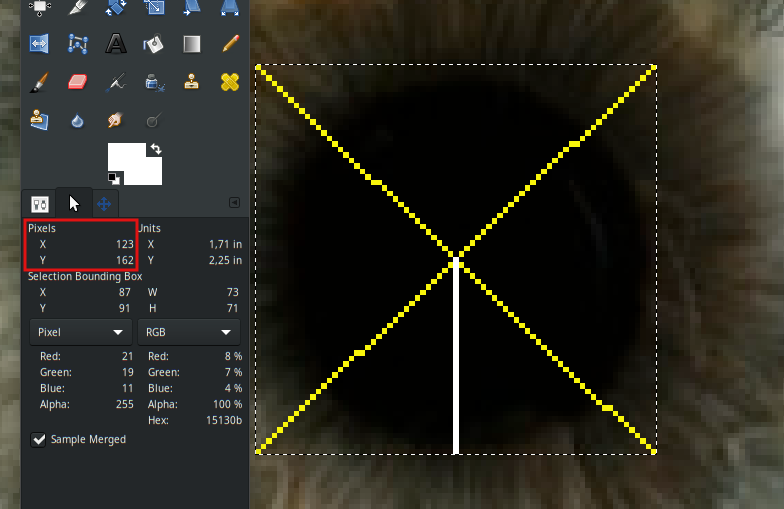
\includegraphics[scale=0.3]{eye2.png}\\
  \caption{Segmento (blanco) recto desde el centro de la pupila hasta un lado del cuadrado}
  \label{fig:rpupil}
\end{figure}

\item Estimación del radio límbico: \textbf{134px}\\
De igual forma que hemos calculado el radio de la pupila podemos calcular el radio límbico, solo hay que extender la selección rectangular de un lado hasta el límite del iris con la esclerótida.

\begin{figure}[h!]
  \centering
  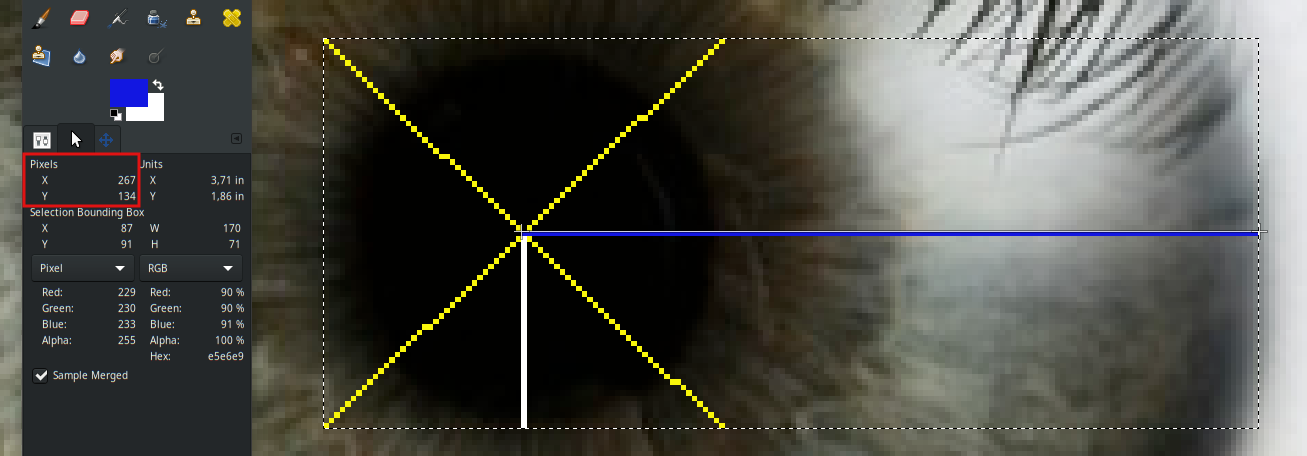
\includegraphics[scale=0.3]{eye3.png}\\
  \caption{Segmento (azul) recto desde el centro de la pupila hasta el límite del iris}
  \label{fig:rlimbic}
\end{figure}
\end{itemize}

\item Considerando las siguientes variables:\\

\begin{center}
$x = 150$

$y = 200$

$x_{0} = 123$

$y_{0} = 126$

$r_{p} = 36px$

$r_{l} = 134px$
\end{center}


El ángulo se calcula como:
\begin{center}
$\alpha = \arctan2(x - x_{0}, y - y_{0})$

$\alpha = \arctan(\frac{y - y_{0}}{x - x_{0}})$

$\alpha = \arctan(\frac{74}{27})$

$\alpha = 1.22 rad$
\end{center}

Para calcular la posición de la coordenada dada en la imagen desenrollada según el formato de Daugman, cada píxel en lugar de definirlo con el sistema de coordenadas cartesiano $(x, y)$ se define en un sistema de coordenadas polar $(r, \alpha)$. Donde $r$ representa el radio dentro del iris y $\alpha$ es el ángulo.\\

El radio $r$ se define como:
\begin{center}
$r = \sqrt{(x - x_{0})^2 + (y - y_{0})^2}$

$r = \sqrt{(27)^2 + (74)^2}$

$r = 78.77px$
\end{center}
Daugman usa los siguientes valores para la imagen normalizada: $M = 256$ y $N = 8$.\\
La coordenada $x'$ en el nuevo sistema de coordenadas polares se calcula como:
\begin{center}
$ x' = \frac{(M-1)(\alpha + \pi)}{2\pi}$

$ x' = \frac{255(1.22 + \pi)}{2\pi}$

$ x' = 156$
\end{center}

La coordenada $y'$ se calcula como:
\begin{center}
$ y' = \frac{(N-1)(r - r_{p})}{r_{l} - r_{p}}$

$ y' = \frac{7(78,77 - 36)}{134 - 36}$

$ y' = 3$
\end{center}
Posición donde irá a parar este punto en la imagen desenrollada según el formato de Daugman:
\begin{center}
$ V(x', y') = (156, 3)$
\end{center}
\end{enumerate}

\pagebreak
\appendix
\section{Características de Haar}
\label{ann:haar}
Este programa hace una extracción de las características de Haar de los conjuntos de imágenes proporcionados (\textit{f} y \textit{n}) y hace el análisis estadístico de las mismas: media y desviación típica.\\
Posteriormente, analiza el conjunto de imágenes a determinar si son cara o no (\textit{c}), aplica las características de Haar de las mismas y determina la probabilidad de que sea una cara o no a través de las funciones probabilísticas.\\

El algoritmo es el siguiente:
\begin{enumerate}
\item Para los dos conjuntos de imágenes proporcionados:
\begin{enumerate}[label=\roman*]
\item Extraer la matriz de la imagen a tratar y pasarla una lista de listas de enteros.
\item Extraer vector $a_{j}^i$: Aplicar los cuatro filtros de Harr sobre la lista y construir una matriz donde las filas correspondes a la característica de Haar (j) y las columnas el número de la imágen al que se le ha aplicado en el conjunto (i).
\item Calcular la media y la desviación típica de cada vector y guardarlo en una lista indexable por número de característica de Haar.
\end{enumerate}
\item Para cada imagen a clasificar del conjunto \textit{c}:
\begin{enumerate}[label=\roman*]
\item Extraer la matriz de la imagen a tratar y pasarla una lista de listas de enteros.
\item Construir vector $cnn_{j}^i$: Aplicar los cuatro filtros de Harr sobre la lista y construir una matriz donde las filas correspondes a la característica de Haar (j) y las columnas el número de la imagen al que se le ha aplicado en el conjunto (i).
\item Para cada valor $j$ del vector $cnn_{j}^i$:
\begin{itemize}
\item Para cada valor $i$ del vector $cnn_{j}^i$:
\begin{enumerate}[label=\roman*]
\item Obtener la media y desviación típica correspondiente a la característica $Haar_{j}$.
\item Obtener la probabilidad a priori de que sea cara $P (x_{i}|``cara'')$ y de que sea no cara $P(x_{i}|``no cara'')$ a partir de la media y la desviación típica proporcionada.
\item Obtener la probabilidad de que sea cara $P_{c}$ y de que sea no cara $P_{nc}$.
\item Si estamos iterando sobre la última carácterística de Haar, obtenemos el producto de las probabilidades de cara y no cara y determinamos la clase a la que pertence el la matriz analizada. Si 
$
  \prod_{i = 1}^{n} P_{i}^c(x_{i}) >  \prod_{i = 1}^{n} P_{i}^{nc}(x_{i})
$ entonces es de la clase ``Cara'', en caso contrario se trata de la clase ``No cara''.
\end{enumerate}
\end{itemize}
\end{enumerate}
\end{enumerate}
\lstinputlisting[language=Python]{haar.py}
\vspace{10px}
\section{Característica de Haar$_{1}$}
\label{ann:haar2}
Versión modificada del programa Filtros de Haar[\ref{ann:haar}] para devolver únicamente resultados de características de Haar$_{1}$.
\lstinputlisting[language=Python, firstline=69, lastline=77]{haar2.py}
\lstinputlisting[language=Python, firstline=118, lastline=125]{haar2.py}

\end{document}